\documentclass[tikz,border=0pt]{standalone}
\usepackage[utf8]{inputenc}
\usepackage[T1]{fontenc}
\usepackage{lmodern}
\usepackage{amsmath,amssymb}
\usetikzlibrary{arrows.meta,positioning,fit,calc,backgrounds,shapes.geometric,decorations.pathreplacing}
\definecolor{navy}{HTML}{163A5F}
\definecolor{blue}{HTML}{2C6EAF}
\definecolor{lightblue}{HTML}{EAF2F8}
\definecolor{midblue}{HTML}{CFE1F2}
\definecolor{graytext}{HTML}{4A5560}
\definecolor{lightgray}{HTML}{F4F6F8}
\definecolor{green}{HTML}{3C8D73}
\definecolor{lightgreen}{HTML}{E8F5EF}
\definecolor{red}{HTML}{B24A4A}
\definecolor{lightred}{HTML}{FBEDEE}
\tikzset{
  title/.style={font=\sffamily\bfseries\fontsize{16}{18}\selectfont,text=navy,anchor=west},
  subtitle/.style={font=\sffamily\bfseries\fontsize{11}{13}\selectfont,text=navy},
  body/.style={font=\sffamily\fontsize{9.2}{11}\selectfont,text=graytext,align=left},
  small/.style={font=\sffamily\fontsize{8}{9.4}\selectfont,text=graytext,align=left},
  tinylabel/.style={font=\sffamily\fontsize{7.2}{8.4}\selectfont,text=graytext},
  panel/.style={rounded corners=3pt,draw=midblue,fill=white,line width=0.6pt},
  box/.style={rounded corners=2pt,draw=midblue,fill=lightblue,line width=0.6pt},
  worker/.style={rounded corners=2pt,draw=blue,dashed,line width=0.7pt,fill=white},
  task/.style={rounded corners=2pt,draw=blue,fill=lightblue,minimum width=0.85cm,minimum height=0.55cm,font=\sffamily\bfseries\small,text=navy},
  file/.style={draw=blue,fill=white,minimum width=0.55cm,minimum height=0.42cm,font=\sffamily\small,text=navy},
  arr/.style={-{Stealth[length=2.4mm,width=1.8mm]},draw=blue,line width=0.9pt},
  arrthin/.style={-{Stealth[length=2mm,width=1.5mm]},draw=blue,line width=0.7pt},
  arrred/.style={-{Stealth[length=2mm,width=1.5mm]},draw=red,dashed,line width=0.8pt},
  arrgreen/.style={-{Stealth[length=2mm,width=1.5mm]},draw=green,dotted,line width=1pt}
}
\begin{document}

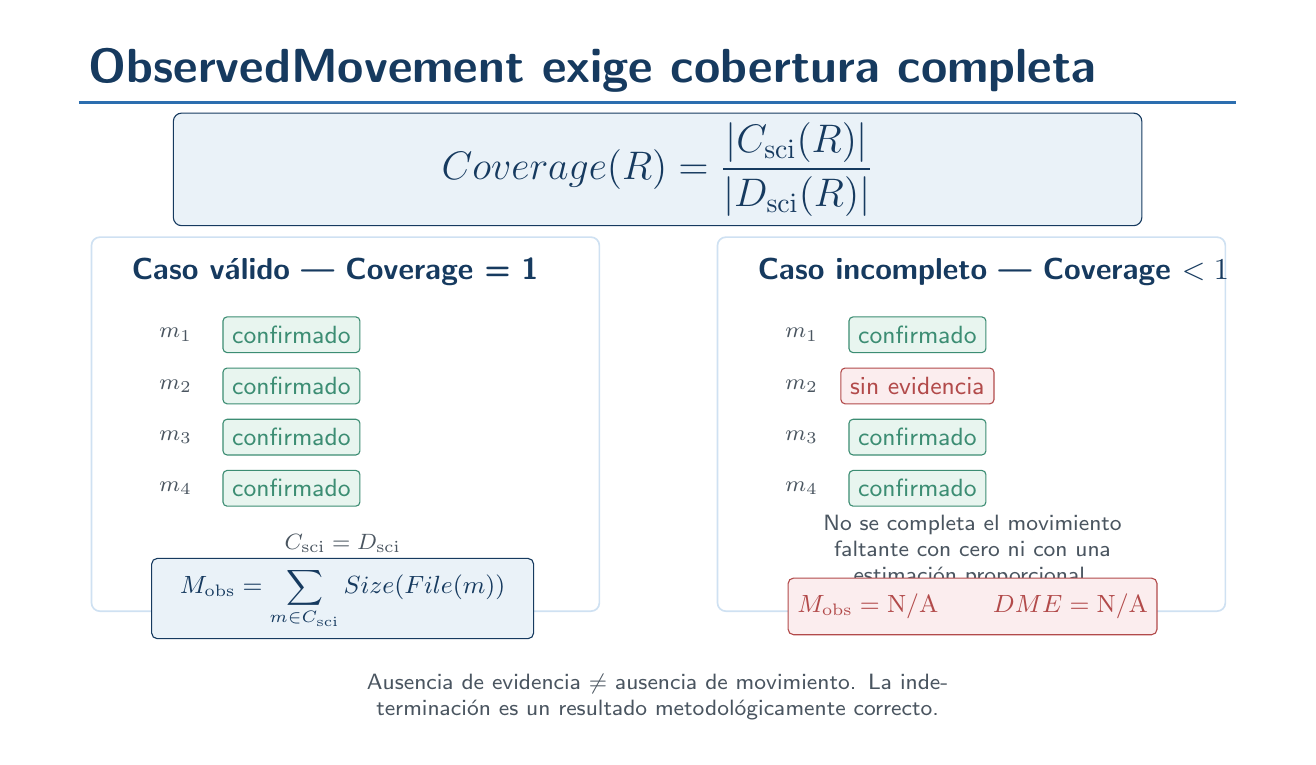
\begin{tikzpicture}[x=1cm,y=1cm]
\path[use as bounding box] (0,0) rectangle (16,9);
\node[title] at (0.65,8.45) {ObservedMovement exige cobertura completa};
\draw[blue,line width=1pt] (0.65,8.05)--(15.35,8.05);
\node[rounded corners=3pt,draw=navy,fill=lightblue,minimum width=12.3cm,minimum height=0.9cm,font=\sffamily\bfseries\Large,text=navy] at (8,7.2) {$Coverage(R)=\dfrac{|C_{\mathrm{sci}}(R)|}{|D_{\mathrm{sci}}(R)|}$};
\node[panel,minimum width=6.45cm,minimum height=4.75cm,anchor=north west] at (0.8,6.35) {};
\node[subtitle,anchor=west] at (1.2,5.9) {Caso válido — Coverage = 1};
\foreach \y/\m in {5.1/$m_1$,4.45/$m_2$,3.8/$m_3$,3.15/$m_4$}{\node[small,anchor=west] at (1.55,\y) {\m}; \node[draw=green,fill=lightgreen,rounded corners=1.5pt,minimum width=1.25cm,minimum height=0.4cm,font=\sffamily\small,text=green] at (3.35,\y) {confirmado};}
\node[small,align=center] at (4.0,2.45) {$C_{\mathrm{sci}}=D_{\mathrm{sci}}$};
\node[rounded corners=2pt,draw=navy,fill=lightblue,minimum width=4.85cm,minimum height=0.72cm,font=\sffamily\bfseries\small,text=navy] at (4.0,1.75) {$M_{\mathrm{obs}}=\displaystyle\sum_{m\in C_{\mathrm{sci}}} Size(File(m))$};
\node[panel,minimum width=6.45cm,minimum height=4.75cm,anchor=north west] at (8.75,6.35) {};
\node[subtitle,anchor=west] at (9.15,5.9) {Caso incompleto — Coverage $<1$};
\node[small,anchor=west] at (9.5,5.1) {$m_1$}; \node[small,anchor=west] at (9.5,4.45) {$m_2$}; \node[small,anchor=west] at (9.5,3.8) {$m_3$}; \node[small,anchor=west] at (9.5,3.15) {$m_4$};
\node[draw=green,fill=lightgreen,rounded corners=1.5pt,minimum width=1.25cm,minimum height=0.4cm,font=\sffamily\small,text=green] at (11.3,5.1) {confirmado};
\node[draw=red,fill=lightred,rounded corners=1.5pt,minimum width=1.55cm,minimum height=0.4cm,font=\sffamily\small,text=red] at (11.3,4.45) {sin evidencia};
\node[draw=green,fill=lightgreen,rounded corners=1.5pt,minimum width=1.25cm,minimum height=0.4cm,font=\sffamily\small,text=green] at (11.3,3.8) {confirmado};
\node[draw=green,fill=lightgreen,rounded corners=1.5pt,minimum width=1.25cm,minimum height=0.4cm,font=\sffamily\small,text=green] at (11.3,3.15) {confirmado};
\node[small,text width=4.6cm,align=center] at (12.0,2.35) {No se completa el movimiento faltante con cero ni con una estimación proporcional.};
\node[rounded corners=2pt,draw=red,fill=lightred,minimum width=4.5cm,minimum height=0.72cm,font=\sffamily\bfseries\small,text=red] at (12.0,1.65) {$M_{\mathrm{obs}}=\mathrm{N/A}\qquad DME=\mathrm{N/A}$};
\node[small,text width=14cm,align=center] at (8,0.5) {Ausencia de evidencia $\neq$ ausencia de movimiento. La indeterminación es un resultado metodológicamente correcto.};
\end{tikzpicture}
\end{document}
